% Options for packages loaded elsewhere
\PassOptionsToPackage{unicode}{hyperref}
\PassOptionsToPackage{hyphens}{url}
%
\documentclass[
]{book}
\usepackage{lmodern}
\usepackage{amssymb,amsmath}
\usepackage{ifxetex,ifluatex}
\ifnum 0\ifxetex 1\fi\ifluatex 1\fi=0 % if pdftex
  \usepackage[T1]{fontenc}
  \usepackage[utf8]{inputenc}
  \usepackage{textcomp} % provide euro and other symbols
\else % if luatex or xetex
  \usepackage{unicode-math}
  \defaultfontfeatures{Scale=MatchLowercase}
  \defaultfontfeatures[\rmfamily]{Ligatures=TeX,Scale=1}
\fi
% Use upquote if available, for straight quotes in verbatim environments
\IfFileExists{upquote.sty}{\usepackage{upquote}}{}
\IfFileExists{microtype.sty}{% use microtype if available
  \usepackage[]{microtype}
  \UseMicrotypeSet[protrusion]{basicmath} % disable protrusion for tt fonts
}{}
\makeatletter
\@ifundefined{KOMAClassName}{% if non-KOMA class
  \IfFileExists{parskip.sty}{%
    \usepackage{parskip}
  }{% else
    \setlength{\parindent}{0pt}
    \setlength{\parskip}{6pt plus 2pt minus 1pt}}
}{% if KOMA class
  \KOMAoptions{parskip=half}}
\makeatother
\usepackage{xcolor}
\IfFileExists{xurl.sty}{\usepackage{xurl}}{} % add URL line breaks if available
\IfFileExists{bookmark.sty}{\usepackage{bookmark}}{\usepackage{hyperref}}
\hypersetup{
  pdftitle={CLEANED Workbook},
  pdfauthor={Jessica Mukiri},
  hidelinks,
  pdfcreator={LaTeX via pandoc}}
\urlstyle{same} % disable monospaced font for URLs
\usepackage{longtable,booktabs}
% Correct order of tables after \paragraph or \subparagraph
\usepackage{etoolbox}
\makeatletter
\patchcmd\longtable{\par}{\if@noskipsec\mbox{}\fi\par}{}{}
\makeatother
% Allow footnotes in longtable head/foot
\IfFileExists{footnotehyper.sty}{\usepackage{footnotehyper}}{\usepackage{footnote}}
\makesavenoteenv{longtable}
\usepackage{graphicx,grffile}
\makeatletter
\def\maxwidth{\ifdim\Gin@nat@width>\linewidth\linewidth\else\Gin@nat@width\fi}
\def\maxheight{\ifdim\Gin@nat@height>\textheight\textheight\else\Gin@nat@height\fi}
\makeatother
% Scale images if necessary, so that they will not overflow the page
% margins by default, and it is still possible to overwrite the defaults
% using explicit options in \includegraphics[width, height, ...]{}
\setkeys{Gin}{width=\maxwidth,height=\maxheight,keepaspectratio}
% Set default figure placement to htbp
\makeatletter
\def\fps@figure{htbp}
\makeatother
\setlength{\emergencystretch}{3em} % prevent overfull lines
\providecommand{\tightlist}{%
  \setlength{\itemsep}{0pt}\setlength{\parskip}{0pt}}
\setcounter{secnumdepth}{5}
\usepackage{booktabs}
\usepackage[]{natbib}
\bibliographystyle{apalike}

\title{CLEANED Workbook}
\author{Jessica Mukiri}
\date{13/05/2020}

\begin{document}
\maketitle

{
\setcounter{tocdepth}{1}
\tableofcontents
}
\hypertarget{preface}{%
\chapter*{Preface}\label{preface}}
\addcontentsline{toc}{chapter}{Preface}

This lab workbook contains hands-on material supplementing the CLEANED training taught by \href{https://jmukiri.com/}{Jessica Mukiri}, An Notenbaert, Birthe Paul, Emmanuel Mwema and Rein Van der Hoek hosted by the \href{https://ciat.cgiar.org/what-we-do/forages-livestock/}{Tropical Forages Program}, at the \href{https://ciat.cgiar.org/alliance/}{Alliance for Bioversity Inventational and CIAT}.

This workbook was written to augment a series of slide deck presentations developed for the training. The slides and workbook, together and along with the virtual presentations, intend to encourage the use of the CLEANED model. Use these resources to guide your learning.

Additionally,how to,videos are integrated into the workbook chapters.The videos also serve to illustrate concepts and techniques not taught in the training.

We hope that you will use and understand the CLEANED model.

\hypertarget{what-you-will-need-to-get-started}{%
\section*{What you will need to get started}\label{what-you-will-need-to-get-started}}
\addcontentsline{toc}{section}{What you will need to get started}

You will need Microsoft Excel 2013 or newer.

You will need to download the model: \href{https://dataverse.harvard.edu/dataset.xhtml?persistentId=doi:10.7910/DVN/G0G8IY}{CLEANED} \& the \href{https://hdl.handle.net/10568/107238}{Manual}

\hypertarget{cleaned-training-introduction-and-information}{%
\chapter{CLEANED Training introduction and information}\label{cleaned-training-introduction-and-information}}

\hypertarget{training-meeting-times}{%
\section{Training Meeting Times}\label{training-meeting-times}}

\begin{itemize}
\tightlist
\item
  Mon, Wed and Fri for virtual training sessions (10:00am -12:00pm: GMT+3)
\item
  Tue and Thu to carry out assignments
\end{itemize}

\hypertarget{prerequisites}{%
\section{Prerequisites}\label{prerequisites}}

There are no prerequisites for this course.

\hypertarget{training-description}{%
\section{Training Description}\label{training-description}}

Livestock are key to food security, nutrition and livelihoods. The demand for livestock products is expected to double in developing countries. However, the livestock sector is also associated with great environmental costs such as land degradation, high water use, excessive GHG emissions and loss of natural ecosystems and biodiversity.

Designing sustainable livestock enterprises poses a challenge in developing countries due to lack of data and models. The CLEANED minimum data ex-ante environmental impact tool developed by the Alliance can help to fill this gap. CLEANED is an easy-to-use Excel-based tool that allows users to explore multiple impacts of developing livestock production systems. It models the impacts of changes in different livestock enterprises on productivity, land and water use, greenhouse gas emissions and soil health.

The aim for this training is to strengthen the technical capacity of agriculture stakeholders and for them to be able to use this tool as a means of improved decision making in the agriculture development sector with a focus on livestock systems.

\hypertarget{learning-outcomes}{%
\section{Learning Outcomes}\label{learning-outcomes}}

If I've done a good job as the instructor and you've put effort into the training, by the end of the two weeks, you will be able to:

\begin{enumerate}
\def\labelenumi{\arabic{enumi}.}
\tightlist
\item
  \textbf{Describe} the importance of carrying out environmental impacts assessments in the livestock sector.
\item
  \textbf{Carry out}assessments using CLEANED and be able to:

  \begin{itemize}
  \tightlist
  \item
    \textbf{Calculate} and gather valid input data needed for the model
  \item
    \textbf{Explain} the calculations and parametrize the tool for a specific enterprise in a specific region
  \item
    \textbf{Carry out} different intervention scenarios
  \end{itemize}
\item
  \textbf{Summarize}, \textbf{analysis} outputs needed for decision making.
\end{enumerate}

\hypertarget{expectations}{%
\section{Expectations}\label{expectations}}

\begin{itemize}
\tightlist
\item
  You are willing to share your knowledge, opinions, and ideas in class.
\item
  You are open to the ideas and knowledge of your peers.
\item
  Any concept that is unclear or confusing will be explored and examined.
\item
  You dedicate yourself to the training and are motivated to learn the model.
\item
  You complete assignments in your own time as they are essential part of the learning.
\end{itemize}

\hypertarget{texts-materials}{%
\section{Texts \& Materials}\label{texts-materials}}

\begin{enumerate}
\def\labelenumi{\arabic{enumi}.}
\tightlist
\item
  Virtual slide presentations and discussions
\item
  Online quizzes
\item
  Pre-recorded materials
\item
  Final assignment and presentation.
\end{enumerate}

\hypertarget{assignments-gradings}{%
\section{Assignments / Grading's}\label{assignments-gradings}}

There are five post-class assignments. Due dates and descriptions are provided in the agenda. These assignments are essential to strengthen your ability to use the CLEANED model.

In addition, each training session will have at least one small group breakout, active learning assignment and independent quizzes.

The grade for this class is either Pass or No record. In order to pass the training, you must satisfactorily complete all of the post-class assignments, and participate in three or more training discussions and activities.

\hypertarget{cleaned-agenda}{%
\section{CLEANED Agenda}\label{cleaned-agenda}}

\begin{figure}
\centering
\includegraphics[width=8.33333in,height=\textheight]{AgendaD123.pdf}
\caption{Agenda}
\end{figure}

\hypertarget{overview-of-cleaned}{%
\chapter{Overview of CLEANED}\label{overview-of-cleaned}}

In this section we shall look at the CLEANED model, what exactly is it?

\hypertarget{slides-recording}{%
\section{Slides \& Recording}\label{slides-recording}}

\textbf{Slides used during day 1}

\textbf{Upload of training video used on day 1}

\hypertarget{quiz-1}{%
\section{Quiz 1}\label{quiz-1}}

\hypertarget{assignment-1}{%
\section{Assignment 1}\label{assignment-1}}

\hypertarget{pre---recorded-materials}{%
\section{Pre - recorded materials}\label{pre---recorded-materials}}

\textbf{Slides and pre-recored voice over}

\emph{for voice over use this link below}

\hypertarget{hands-on-with-the-input-section}{%
\chapter{Hands-on with the INPUT section}\label{hands-on-with-the-input-section}}

In this section we shall look at the INPUT section of the CLEANED model.

\hypertarget{slides-recording}{%
\section{Slides \& Recording}\label{slides-recording}}

\textbf{Slides used during day 2}

\textbf{Upload of training video used on day 2}

\hypertarget{quiz-2}{%
\section{Quiz 2}\label{quiz-2}}

\hypertarget{assignment-2}{%
\section{Assignment 2}\label{assignment-2}}

\hypertarget{pre---recorded-materials}{%
\section{Pre - recorded materials}\label{pre---recorded-materials}}

\textbf{Slides used for the pre-recorded videos}

\textbf{Upload of pre- recorded video material}

\hypertarget{outputs-and-results}{%
\chapter{Outputs and Results}\label{outputs-and-results}}

In this section we shall look at the Results section of the CLEANED model.

\hypertarget{slides-recording}{%
\section{Slides \& Recording}\label{slides-recording}}

\textbf{Slides used during day 3}

\textbf{Upload of training video used on day 3}

\hypertarget{quiz-3}{%
\section{Quiz 3}\label{quiz-3}}

\hypertarget{assignment-3}{%
\section{Assignment 3}\label{assignment-3}}

\hypertarget{pre---recorded-materials}{%
\section{Pre - recorded materials}\label{pre---recorded-materials}}

\textbf{Slides used for the pre-recorded videos}

\textbf{Upload of pre- recorded video material}

\hypertarget{examples-of-cleaned-outputs}{%
\section{Examples of CLEANED Outputs}\label{examples-of-cleaned-outputs}}

\begin{figure}
\centering
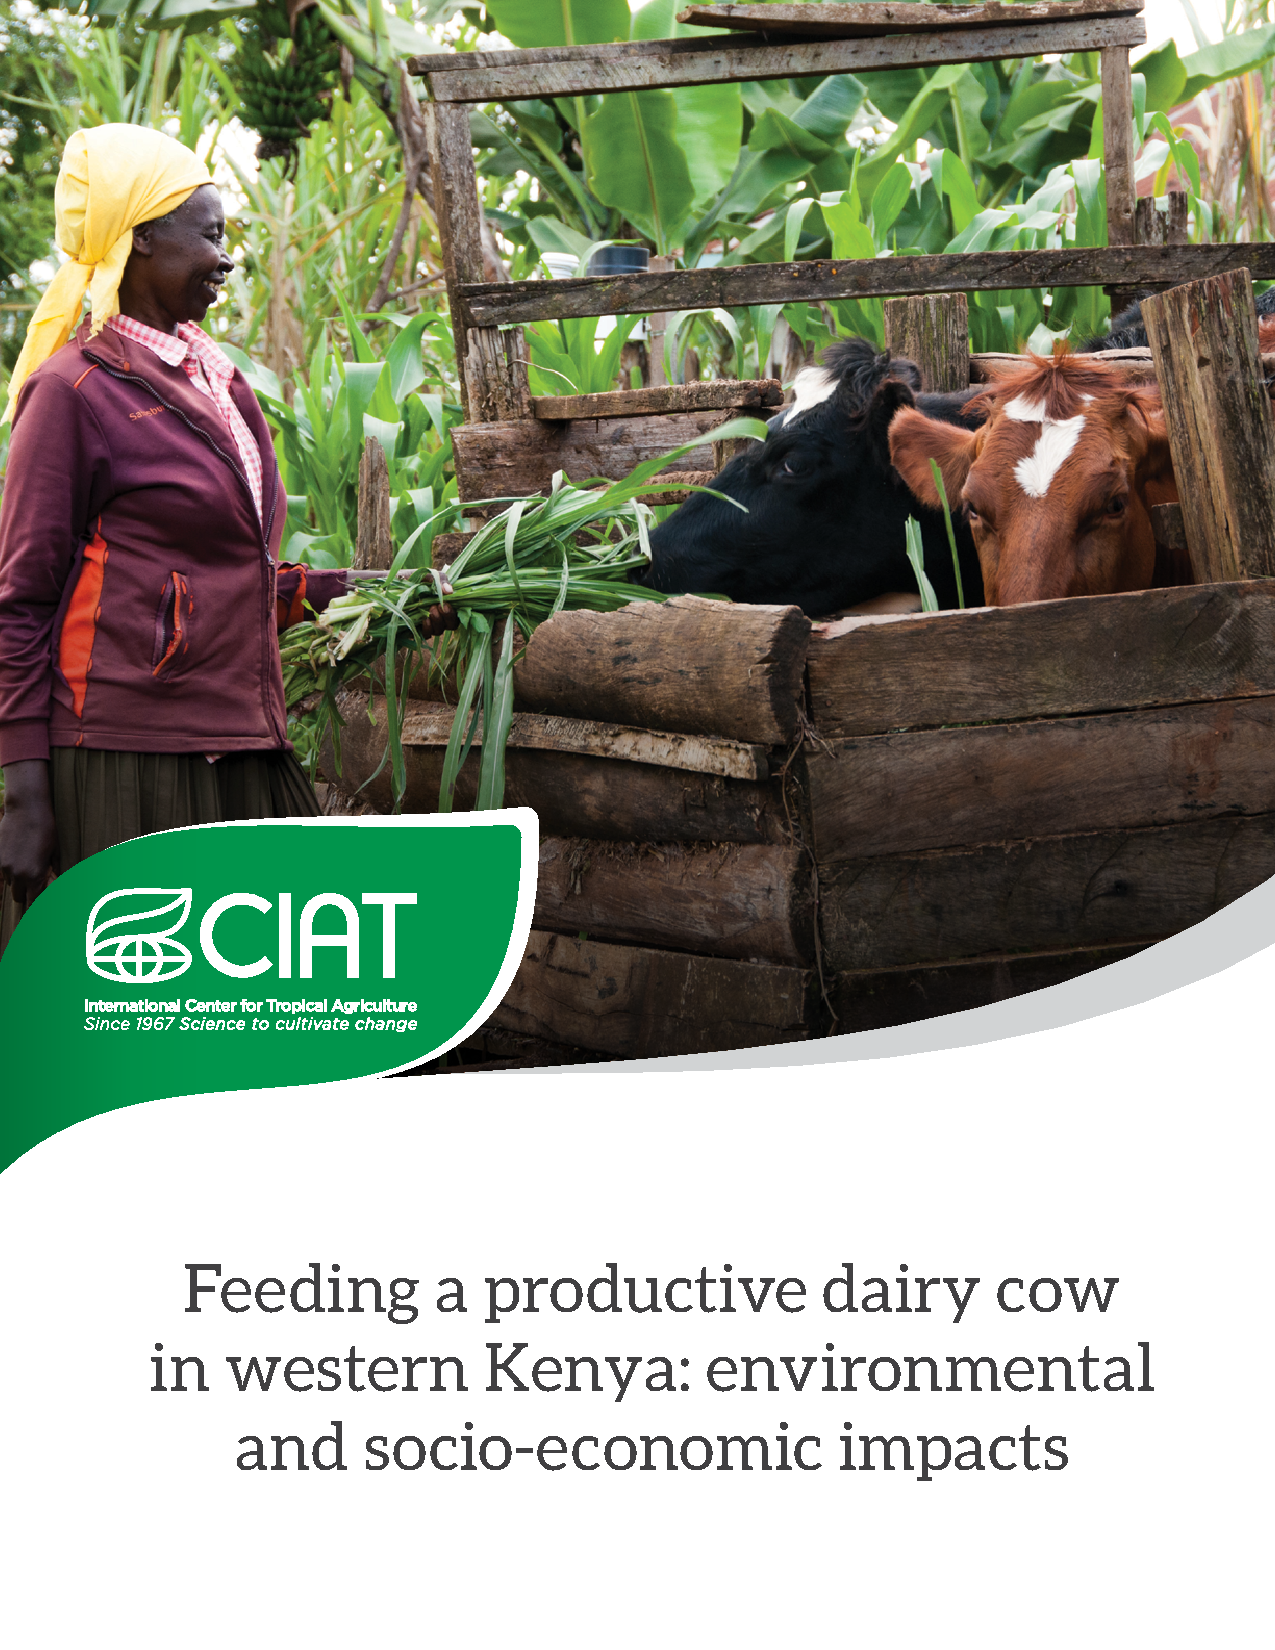
\includegraphics[width=5.20833in,height=\textheight]{FEEDING A PRODUCTIVE DAIRY COW IN WESTERN KENYA.pdf}
\caption{Feeding a productive dairy cow in western Kenya: environmental and socioeconomic impacts}
\end{figure}

\hypertarget{paramters-calculations-for-impacts}{%
\chapter{Paramters + Calculations for impacts}\label{paramters-calculations-for-impacts}}

In this section we shall look at the several dimensions of the CLEANED model.

\hypertarget{slides-recording}{%
\section{Slides \& Recording}\label{slides-recording}}

\textbf{Slides used during day 4}

\textbf{Upload of training video used on day 4}

\hypertarget{quiz-4}{%
\section{Quiz 4}\label{quiz-4}}

\hypertarget{assignment-4}{%
\section{Assignment 4}\label{assignment-4}}

\hypertarget{pre---recorded-materials}{%
\section{Pre - recorded materials}\label{pre---recorded-materials}}

\textbf{Upload of pre- recorded video material}

\hypertarget{paramters-calculations-for-impacts}{%
\chapter{Paramters + Calculations for impacts}\label{paramters-calculations-for-impacts}}

In this section we shall look at the several dimensions of the CLEANED model.

\hypertarget{slides-recording}{%
\section{Slides \& Recording}\label{slides-recording}}

\textbf{Slides used during day 5}

\textbf{Upload of training video used on day 5}

\hypertarget{quiz-5}{%
\section{Quiz 5}\label{quiz-5}}

\hypertarget{final-assigment}{%
\section{Final assigment}\label{final-assigment}}

\hypertarget{cleaned-tutorials}{%
\chapter*{CLEANED tutorials}\label{cleaned-tutorials}}
\addcontentsline{toc}{chapter}{CLEANED tutorials}

\emph{How to add a feed item}

  \bibliography{book.bib,packages.bib}

\end{document}
